\lecture{18}{30 aprile 2024}
\section{Propagazione nei materiali}
Per i materiali la velocità è \(\quotient{1}{\sqrt{\mu \varepsilon } } \), che nella maggior parte dei casi si riduce a \(\quotient{c}{\sqrt{\varepsilon _r} }=\quotient{c}{n} \) perché \(\mu _r \thickapprox 1\) (i mezzi così sono detti mezzi ottici).
\begin{definition}
	[Indice di rifrazione]
	\begin{equation}
		n = \frac{c}{v} \thickapprox \sqrt{\varepsilon _r}  \geq 1
	\end{equation}
\end{definition}
Considerando la luce che viaggia in acqua (\(\varepsilon _r \thickapprox 80\)), trovo che la velocità della luce dovrebbe essere \(v\thickapprox \quotient{c}{9} \), mentre se faccio una misura trovo \(v \thickapprox \quotient{3}{4} c\). La soluzione potrebbe essere che la costante dielettrica relativa varia al passaggio di un'onda elettromagnetica! Nei mezzi ottici, senza cariche e senza correnti, \(\vert \vec{E} \vert = v \vert \vec{B} \vert = v \mu \vert \vec{H} \vert \). Inoltre
\begin{figure}[H]
	\centering
	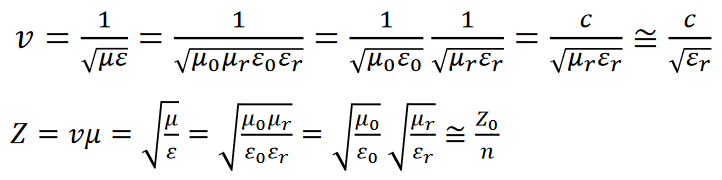
\includegraphics[width=0.5\textwidth]{screenshots/2024-04-30-11-26-26.png}
\end{figure}

\subsection{Cosa succede nei dielettrici?}
Considero un mezzo dielettrico fra le lastre di un condensatore:
\begin{figure}[H]
	\centering
	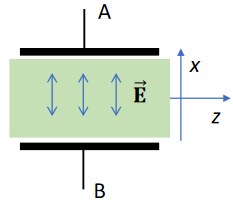
\includegraphics[width=0.3\textwidth]{screenshots/2024-04-30-11-33-08.png}
\end{figure}
Detta \(V_0\) la differenza di potenziale applicata alle lastre del condensatore, il campo elettrico senza dielettrico sarà \(\vert \vec{E} \vert = \quotient{V_0}{d} \) e in presenza di dielettrico sarà \(\vert \vec{E} \vert = \quotient{\vert \vec{E}_0 \vert }{\varepsilon _r}\). Il campo elettrico deforma le molecole e nasce un momento di dipolo indotto: \(\vec{p}= \alpha \vec{E}\) dove \(\alpha \) è la polarizzabilità atomica/molecolare. È come se ogni atomo sentisse una forza elettrica approssimabile \(\vec{f}= q \vec{E}\), in modo che le forze interne rispondano con una forza elastica \(f_e = -kx\).

Consideriamo ora cosa succede quando il potenziale è variabile: \(\Delta V (t) = V_0 \cos (\omega t)\). L'asse x è diretto come il campo elettrico e ha origine sull'atomo. L'elettrone si comporta come un oscillatore armonico forzato. Sia \(f=-kx\) la forza di richiamo elastica, \(f_v = -\beta \dot{x}\) la forza viscosa e \( =E_0 e^{i \omega t}\) l'andamento del campo elettrico.
\begin{equation}
	m \ddot{x} + \beta \dot{x} + kx = - e E_0 e^{i \omega t}
\end{equation}
Poniamo \(\gamma = \quotient{\beta }{m}, \omega _0 ^{2} = \quotient{k}{m} \). Siamo bravissimi e sappiamo già risolvere questo problema! (Guardiamo solo la soluzione stazionaria quando il transiente non ha più effetto).
\begin{equation}
	x(t)= A e^{i \omega t} \text{ con } A= \frac{-e E_0}{m[(- \omega ^{2} + \omega ^{2} _0) + i \gamma \omega ]}
\end{equation}
Ma a livello macroscopico cosa succede? Ogni atomo ha un dipolo atomico \(\vec{p}=-e x \vec{\hat{i}}\). La polarizzazione del dielettrico è \(\vec{P}= n_a \vec{p}\) dove \(n_a\) è la densità atomica. Da elettromagnetismo sappiamo che c'è una relazione fra \(\vec{P}\) ed \(\vec{E}\): \(\vec{P}= \varepsilon _0 \chi _e \vec{E} = \varepsilon _0 \chi _e E_0 e^{i \omega t} \vec{\hat{i}}\). Dalla soluzione precedente ho anche:
\begin{align}
	\vec{P}&= \varepsilon _0 \chi _e \vec{E} = n_a \vec{p} = -e n_a x(t) \vec{i}=\\
	&= - e n_a \frac{- e E_0}{m[(- \omega ^{2} + \omega ^{2} _0) + i \gamma \omega ]}e^{i \omega t} \vec{\hat{i}}
\end{align}
Da cui posso risolvere per \(\chi _e\) (la suscettività elettrica del materiale):
\begin{figure}[H]
	\centering
	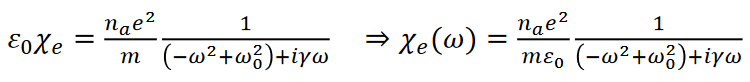
\includegraphics[width=0.5\textwidth]{screenshots/2024-04-30-11-45-24.png}
\end{figure}
Da cui si ottiene che \(\varepsilon (\omega )= \varepsilon _0 + \varepsilon _0 \chi _e(\omega )\) e l'indice di rifrazione che sarà:
\begin{align}
	n (\omega ) &= \sqrt{\varepsilon _r (\omega )} = \sqrt{1 + \chi _e (\omega )} \thickapprox 1 + \frac{1}{2}\chi _e(\omega )\\
	&= 1 + \frac{n_a e^{2} }{2 m \varepsilon _0} \frac{1}{(-\omega ^{2} + \omega ^{2} _0)+ i \gamma \omega }
\end{align}
L'indice di rifrazione ha una componente immaginaria, possiamo scriverlo come \(n(\omega ) = n_r - i n_I\) con
\begin{figure}[H]
	\centering
	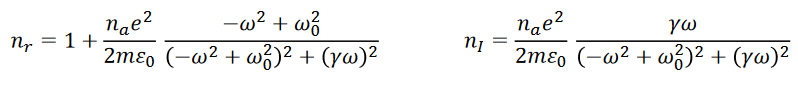
\includegraphics[width=0.5\textwidth]{screenshots/2024-04-30-11-49-36.png}
\end{figure}
La parte reale dell'indice di rifrazione dipende dalla pulsazione, quindi la velocità di fase dipende dalla pulsazione dell'onda e il mezzo è dispersivo! Anche \(k\) dipende dall'indice di rifrazione:
\begin{figure}[H]
	\centering
	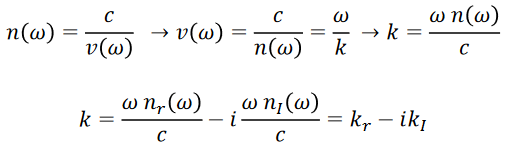
\includegraphics[width=0.4\textwidth]{screenshots/2024-04-30-11-50-50.png}
\end{figure}
\paragraph{Legge di Lambert}
Che significato ha il numero d'onda complesso \(k= k_r - i k_I\)? Considero un'onda elettrica che si propaga nella direzione z e che oscilla come il campo elettrico di prima: \(E(z,t) = E_0 e^{i( \omega t - kz)}\).
\begin{figure}[H]
	\centering
	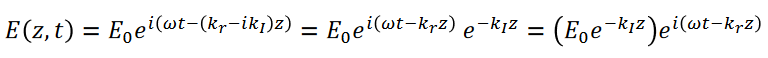
\includegraphics[width=0.5\textwidth]{screenshots/2024-04-30-11-53-50.png}
\end{figure}
L'onda appare muoversi con una velocità \(v= \quotient{\omega }{k_r} = \quotient{c}{n_r} \), ma la sua ampiezza si riduce man mano che avanza nel mezzo dielettrico. Pongo \(\beta = k_I\), l'ampiezza cala come \(E_0(z)=E_0 e^{-\beta z}\). L'intensità dell'onda cambia con il progredire dell'onda nel mezzo (\(I \propto E_0 ^{2} \)):
\begin{formula}
	[Legge di Lambert]
	\begin{equation}
		I(z) = I_0 e^{-2 \beta z} = I_0 e^{- \mu z}
	\end{equation}
	dove si è posto \(\mu = 2 \beta \) che è detto \emph{coefficiente di assorbimento}.
\end{formula}
La dissipazione di energia è dovuta al termine viscoso dell'oscillatore forzato usato nel modellino.

\paragraph{Velocità di gruppo}
Essendo in un mezzo dispersivo, la velocità di fase e la velocità di gruppo saranno diverse. La velocità di gruppo si trova come segue:
\begin{figure}[H]
	\centering
	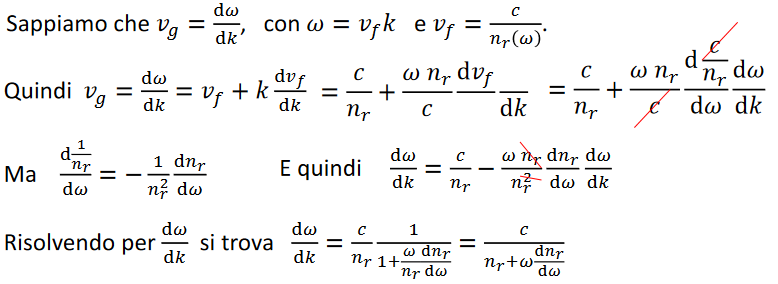
\includegraphics[width=0.5\textwidth]{screenshots/2024-04-30-12-00-57.png}
\end{figure}
\begin{remark}
	Si possono avere due casi di dispersione: la dispersione normale e la dispersione anomala. Nel primo caso, \(\frac{\mathrm{d}n_r}{\mathrm{d}\omega } \geq 0 \implies v_g \leq v_f\), mentre nel secondo \(\frac{\mathrm{d}n_r}{\mathrm{d}\omega } \implies v_g \geq v_f \).
\end{remark}
Si possono studiare gli andamenti della parte reale e immaginaria dell'indice di rifrazione di un singolo elettrone:
\begin{figure}[H]
	\centering
	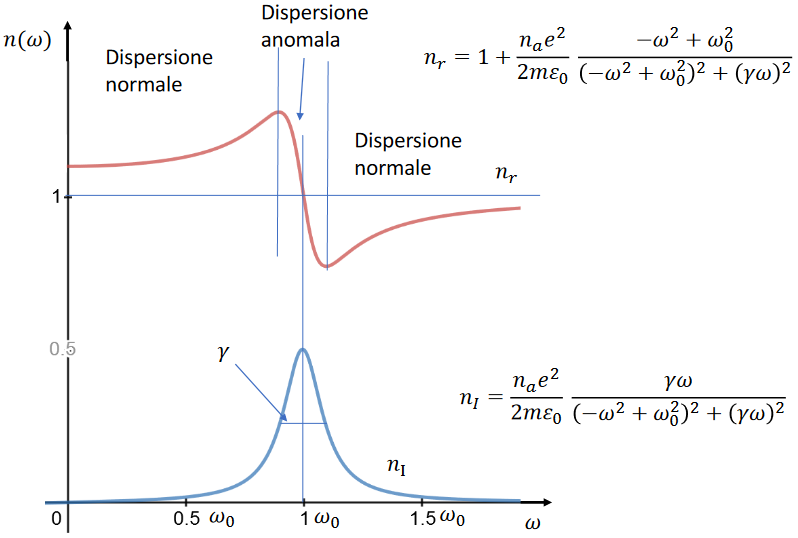
\includegraphics[width=0.5\textwidth]{screenshots/2024-04-30-12-05-26.png}
\end{figure}
% TODO mettere reference per ampiezze
Ricordano molto l'ampiezza elastica e l'ampiezza assorbitiva! La regione del picco nella parte immaginaria dell'indice di rifrazione indica la regione in cui l'energia viene maggiormente assorbita dal materiale e quindi in cui l'onda fa più fatica ad attraversarlo. Notiamo che questi andamenti descrivono un atomo di idrogeno con un singolo elettrone. Nel caso generico in cui un atomo può avere più elettroni con diverse pulsazioni proprie si generalizza come segue:
\begin{figure}[H]
	\centering
	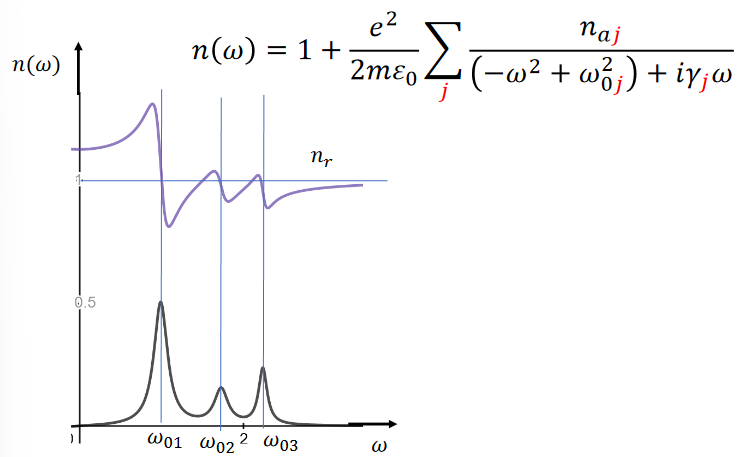
\includegraphics[width=0.45\textwidth]{screenshots/2024-04-30-12-08-10.png}
\end{figure}
Si nota che ad alte pulsazioni l'indice di rifrazione si avvicina a 1.

\paragraph{Limite delle alte frequenze}
Consideriamo il caso \(\omega \gg \omega _{0j} \forall j\), cioè il limite di raggi X energetici o raggi gamma:
\begin{figure}[H]
	\centering
	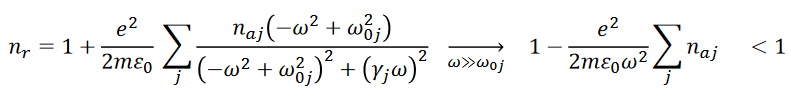
\includegraphics[width=0.5\textwidth]{screenshots/2024-04-30-12-12-53.png}
\end{figure}
Quindi si trova che la velocità di fase è maggiore di \(c\)!
\begin{equation}
	v_f = \frac{c}{n_r} = \frac{c}{1- \frac{e^{2} }{2m \varepsilon _0 \omega ^{2} }\sum_{j}n_{aj} } > c
\end{equation}
Ma ci salviamo in corner: l'importante è che la velocità a cui viaggia l'informazione sia minore di \(c\). Per fortuna è questo il caso:
\begin{equation}
	n_r(\omega )=1- \frac{e^{2} }{2 m \varepsilon _0 \omega ^{2} }\sum_{j} n_{aj} \rightsquigarrow \frac{\mathrm{d}n_r}{\mathrm{d}\omega } = \frac{e ^{2} }{m \varepsilon _0 \omega ^{3}} \sum_{j}n_{aj}    
\end{equation}
da cui
\begin{figure}[H]
	\centering
	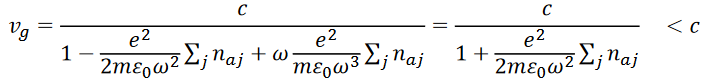
\includegraphics[width=0.5\textwidth]{screenshots/2024-04-30-12-16-51.png}
\end{figure}

\subsection{Propagazione in un metallo}
Possiamo assumere il metallo come neutro, quindi \(\rho =0\). Però esistono cariche libere che danno origine a una corrente: \(\vec{J}= \sigma \vec{E}\).
\begin{figure}[H]
	\centering
	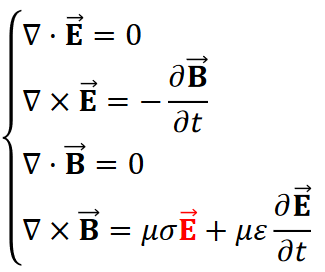
\includegraphics[width=0.4\textwidth]{screenshots/2024-04-30-12-30-10.png}
\end{figure}
Sono equazioni lineari e omogenee, ottimo. Possiamo estrarre anche da qui l'equazione di D'Alembert?
\begin{gather}
	\curl{(\curl{\vec{E}} )} = \curl{(-\frac{\partial \vec{B}}{\partial t} )} = - \frac{\partial (\curl{\vec{B}} )}{\partial t}\\
	\grad{(\div{\vec{E}} )} - \laplacian{\vec{E}} = - \mu \sigma \frac{\partial \vec{E}}{\partial t} - \mu \varepsilon \frac{\partial ^{2} \vec{E}}{\partial t^{2} }\\
	\laplacian{\vec{E}}=\mu \varepsilon \frac{\partial ^{2} \vec{E}}{\partial t^{2} }+\mu \sigma \frac{\partial \vec{E}}{\partial t}    
\end{gather}
Non è l'equazione di D'Alembert, quindi sono in un mezzo dispersivo. La ritrovo solo nel limite \(\sigma \to 0\). Cerchiamo una soluzione nella forma di onde piane armoniche:
\begin{align}
	\vec{E}(\vec{r},t) &= \vec{E}_0 e^{i(\vec{k}\cdot \vec{r} - \omega t)} & \vec{B}(\vec{r},t)&= \vec{B}_0 e^{i (\vec{k}\cdot \vec{r}-\omega t)}
\end{align}
Così le equazioni di Maxwell assumono questa forma:
\begin{figure}[H]
	\centering
	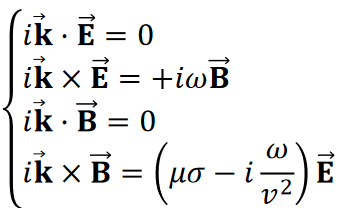
\includegraphics[width=0.4\textwidth]{screenshots/2024-04-30-12-39-14.png}
\end{figure}
\(\vec{E} \perp \vec{k},\ \vec{B}\perp \vec{k}\) quindi le onde in un metallo sono ancora onde trasversali. Inoltre \(\vec{E}\perp \vec{B}\), ma in generale non sono in fase perché c'è un numero complesso come proporzionalità fra i due. Significa che il vettore \(\vec{k}\) contiene una fase complessa. Provo a ricavare la componente complessa di \(\vec{k}\).
\begin{equation}
	i \vec{k} \cp \vec{B} = i \vec{k} \cp \frac{\vec{k}\cp \vec{E}}{\omega } = \frac{i}{\omega } [(\vec{k} \cdot \vec{E})\vec{k} - (\vec{k}\cdot \vec{k})\vec{E}] = -\frac{ik^{2} }{\omega }\vec{E}
\end{equation}
Inoltre avevo
\begin{equation}
	i \vec{k}\cp \vec{B}=\left( \mu \sigma - i \frac{\omega }{v^{2} } \right)\vec{E} 
\end{equation}
da cui
\begin{gather}
	-\frac{i k^{2} }{\omega } = \left( \mu \sigma - i \frac{\omega }{v^{2} } \right) \implies k^{2} = \frac{\omega ^{2} }{v ^{2} } + i \mu  \sigma  \omega = \frac{\omega ^{2} }{v^{2} }\left( 1+ i \frac{\mu \sigma v^{2} }{\omega } \right) \implies \\
	\implies k = \frac{\omega }{v}\sqrt{1+ i \frac{\mu \sigma v^{2} }{\omega }} = k_r + i k_I 
\end{gather}
Anche qui noto che per \(\sigma \to 0\) riottengo una relazione già vista per le onde elettromagnetiche nel vuoto (\(k=\quotient{\omega }{v} \)). Il segno che compare di fronte a \(k_I\) è una convenzione: se avessimo usato un'onda con fase \(\omega t - \vec{k}\cdot \vec{r}\) avremmo ottenuto \(k=k_r - ik_I\).

\paragraph{Assorbimento dell'onda nel metallo}
Consideriamo un'onda che si propaga nella direzione delle z positive e che incontra un metallo per \(z>0\):
\begin{figure}[H]
	\centering
	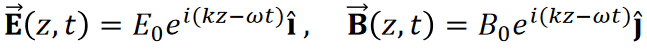
\includegraphics[width=0.4\textwidth]{screenshots/2024-04-30-12-51-51.png}
\end{figure}
Il campo elettrico risulta
\begin{figure}[H]
	\centering
	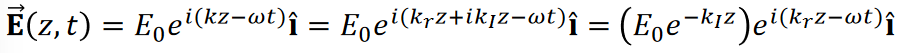
\includegraphics[width=0.5\textwidth]{screenshots/2024-04-30-12-52-15.png}
\end{figure}
L'onda nel metallo ha un'ampiezza decrescente con la profondità (perde energia!). La parte immaginaria di \(k\) descrive l'assorbimento progressivo, dovuto alla perdita di energia per la messa in moto delle cariche. L'energia si trasferisce dall'onda al metallo, si ha il cosiddetto "effetto Joule". Come per le onde in un dielettrico, si definisce il coefficiente di assorbimento \(\mu = 2k_I\). Così \(I(z)=I_0 e^{-\mu z}\).
\begin{figure}[H]
	\centering
	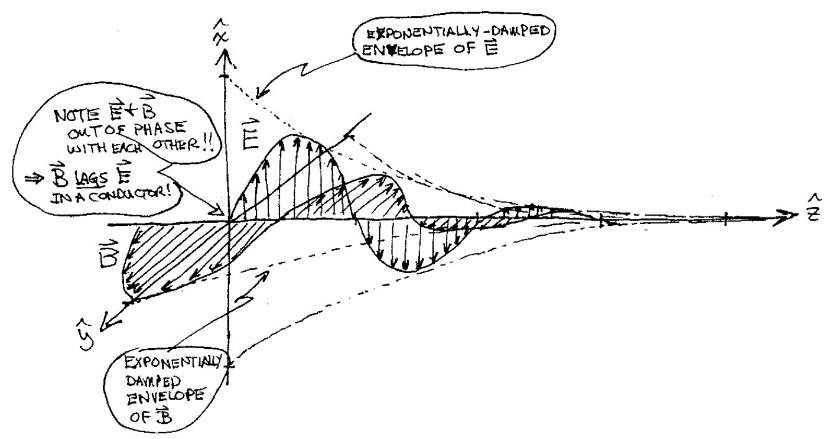
\includegraphics[width=0.5\textwidth]{screenshots/2024-04-30-12-56-12.png}
\end{figure}
Dalla figura si vede che il campo magnetico è sempre in ritardo rispetto al campo elettrico e che entrambe le onde sono attenuate nel tempo.